%%%%%%%%%%%%%%%%%%%%%%%%%%%%%%%%%%%%%%%%%
% Beamer Presentation
% LaTeX Template
% Version 1.0 (10/11/12)
%
% This template has been downloaded from:
% http://www.LaTeXTemplates.com
%
% License:
% CC BY-NC-SA 3.0 (http://creativecommons.org/licenses/by-nc-sa/3.0/)
%
%%%%%%%%%%%%%%%%%%%%%%%%%%%%%%%%%%%%%%%%%

%----------------------------------------------------------------------------------------
%	PACKAGES AND THEMES
%----------------------------------------------------------------------------------------

\documentclass[slidestop,compress,11pt,xcolor=dvipsnames]{beamer}

\mode<presentation> {

% The Beamer class comes with a number of default slide themes
% which change the colors and layouts of slides. Below this is a list
% of all the themes, uncomment each in turn to see what they look like.

%\usetheme{default}
%\usetheme{AnnArbor}
%\usetheme{Antibes}
%\usetheme{Bergen}
%\usetheme{Berkeley}
%\usetheme{Berlin}
%\usetheme{Boadilla}
%\usetheme{CambridgeUS}
%\usetheme{Copenhagen}
%\usetheme{Darmstadt}
%\usetheme{Dresden}
%\usetheme{Frankfurt}
%\usetheme{Goettingen}
%\usetheme{Hannover}
%\usetheme{Ilmenau}
%\usetheme{JuanLesPins}
%\usetheme{Luebeck}
\usetheme{Madrid}
%\usetheme{Malmoe}
%\usetheme{Marburg}
%\usetheme{Montpellier}
%\usetheme{PaloAlto}
%\usetheme{Pittsburgh}
%\usetheme{Rochester}
%\usetheme{Singapore}
%\usetheme{Szeged}
%\usetheme{Warsaw}

% As well as themes, the Beamer class has a number of color themes
% for any slide theme. Uncomment each of these in turn to see how it
% changes the colors of your current slide theme.

%\usecolortheme{albatross}
%\usecolortheme{beaver}
%\usecolortheme{beetle}
\usecolortheme{crane}
%\usecolortheme{dolphin}
%\usecolortheme{dove}
%\usecolortheme{fly}
%\usecolortheme{lily}
%\usecolortheme{orchid}
%\usecolortheme{rose}
%\usecolortheme{seagull}
%\usecolortheme{seahorse}
%\usecolortheme{whale}
%\usecolortheme{wolverine}

%\setbeamertemplate{footline} % To remove the footer line in all slides uncomment this line
%\setbeamertemplate{footline}[page number] % To replace the footer line in all slides with a simple slide count uncomment this line

%\setbeamertemplate{navigation symbols}{} % To remove the navigation symbols from the bottom of all slides uncomment this line
}

\usepackage{graphicx} % Allows including images
\usepackage{booktabs} % Allows the use of \toprule, \midrule and \bottomrule in tables
 \usepackage{url}
\usepackage{relsize}
\usepackage{amsmath}
\usepackage{float}
\usepackage[utf8]{inputenc}
\usepackage[T1]{fontenc}
 \usepackage{booktabs}
 \usepackage{url}
 \usepackage{graphicx}
\usepackage{relsize}
\usepackage{amsmath}
\usepackage{float}


\usefonttheme[onlymath]{serif}
\definecolor{LHCblue}{RGB}{4, 114, 255}
\usecolortheme[named=LHCblue]{structure}
\usepackage{multicol}
\usepackage{lmodern}
\usepackage{lipsum}
\usepackage{marvosym}
\usepackage{graphicx}
\graphicspath{ {images/} }

%----------------------------------------------------------------------------------------
%	TITLE PAGE
%----------------------------------------------------------------------------------------

\title[Author Profiling]{Author Profiling} % The short title appears at the bottom of every slide, the full title is only on the title page

\author{Borna Sirovica,Filip Zelić,Ivan-Dominik Ljubičić} % Your name
\institute[FER] % Your institution as it will appear on the bottom of every slide, may be shorthand to save space
{
Fakultet elektrotehnike i računarstva \\ % Your institution for the title page
\medskip

}
\date{\today} % Date, can be changed to a custom date

\begin{document}

\begin{frame}
\titlepage % Print the title page as the first slide
\end{frame}

\begin{frame}
\frametitle{Content} % Table of contents slide, comment this block out to remove it
\tableofcontents % Throughout your presentation, if you choose to use \section{} and \subsection{} commands, these will automatically be printed on this slide as an overview of your presentation
\end{frame}

%----------------------------------------------------------------------------------------
%	PRESENTATION SLIDES
%----------------------------------------------------------------------------------------

%------------------------------------------------
\section{Project topic} % Sections can be created in order to organize your presentation into discrete blocks, all sections and subsections are automatically printed in the table of contents as an overview of the talk
%------------------------------------------------

\begin{frame}
\frametitle{Author Profiling}
\begin{itemize}
	\item Identifying information about an author by analyzing their writing style
	\item Distinguishes between classes of authors studying their sociolect aspect
	\item Growing importance in forensics, security, marketing, and social networks
\end{itemize}
	\vspace{3mm}
	\centerline{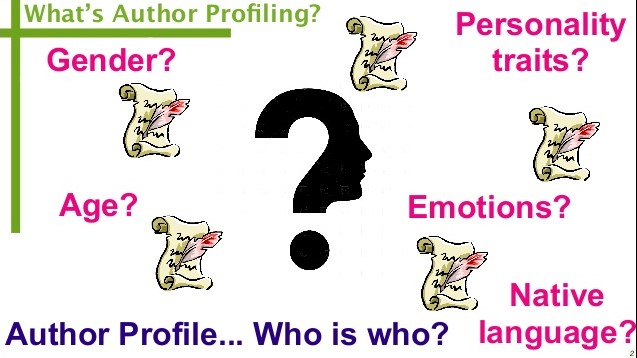
\includegraphics[scale=0.35]{author-profiling-task}}

\end{frame}


%------------------------------------------------

\begin{frame}
\frametitle{Our task}
\vspace{-2mm}
\begin{itemize}
\setlength\itemsep{2mm}
	\item Predicting author profiling aspects
	\begin{itemize}
		\item Demographics (Classification)
		\begin{itemize}
			\item age
			\item gender
		\end{itemize}
		\item Big Five personality traits (Regression)
		\begin{itemize}
			\item extroversion
			\item stability
			\item agreeableness
			\item conscientiousness
			\item openness
		\end{itemize}
	\end{itemize}
\end{itemize}
\end{frame}



%------------------------------------------------

%------------------------------------------------
\section{Dataset}
%------------------------------------------------

%------------------------------------------------

\begin{frame}
\frametitle{Dataset}
\begin{itemize}
	\item English tweets dataset from PAN 2015 competition
	\begin{itemize}
			\item XML format, 152 users
			\item Age and gender labels
			\begin{itemize}
				\item 18-24, 25-34 35-49, 50+
				\item M, F
			\end{itemize}
			\item Personality traits
			\begin{itemize}
				\item normalized numeric rating in [-0.5,0.5] range
			\end{itemize}
		\end{itemize}
\end{itemize}
\vspace{2mm}
\centerline{
\includegraphics[scale=0.5]{twitter-gender}}
\end{frame}

%------------------------------------------------

%------------------------------------------------
\section{Preprocessing}
%------------------------------------------------

%------------------------------------------------

\begin{frame}
\frametitle{Preprocessing}
\begin{itemize}
	\item Creating a document of tweets for each user
	\item Cleaning tweets from
	\begin{itemize}
		\item XML tags
		\item hashtags
		\item @mentions
		\item URLs
		\item stop words		
		\item duplicates
		
	\end{itemize}
	\vspace{-8mm}
	\centerline{
\includegraphics[scale=0.3]{cleaning}}
\end{itemize}
\end{frame}

%------------------------------------------------
\section{Feature extraction}
%------------------------------------------------


\begin{frame}
\frametitle{Feature extraction}
\begin{itemize}
	\item Custom designed features
	\item Extracted from publicly available resources
\end{itemize}
	\vspace{4mm}
	\centerline{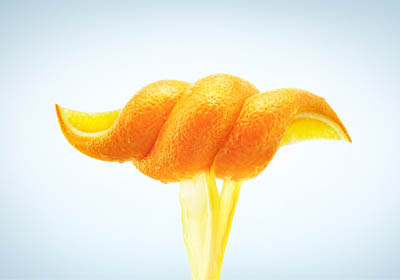
\includegraphics[scale=0.5]{orange}}
\end{frame}


\begin{frame}
\frametitle{Features}
\begin{itemize}
	\setlength\itemsep{2mm}
	\item Lexicon Features
	\begin{itemize}
		\item NRC Word-Emotion Association Lexicon
		\item Internet slang word lexicon
		\item Frequent male and female words lexicon
		\item Frequent male and female function words lexicon
	\end{itemize}
	\item Twitter-specific Features
	\begin{itemize}
		\item hashtags
		\item URLs
		\item user mentions
		\item emoticons
	\end{itemize}
\end{itemize}
	
\end{frame}

\begin{frame}
\frametitle{Features (cont'd)}
\begin{itemize}
	\setlength\itemsep{2mm}
	\item Ortographic Features
	\begin{itemize}
		\item letter case
		\item character flooding
		\item word length
		\item tweet length
		\item specific characters (exclamation points, question marks, apostrophes...)
	\end{itemize}
	\item Term-level Features
	\begin{itemize}
		\item n-grams (TF-IDF matrices of unigrams and trigrams)
		\item F-score
	\end{itemize}
\end{itemize}
\end{frame}

%------------------------------------------------
\section{Supervised learning models}
%------------------------------------------------

\begin{frame}
\centering
\frametitle{Machine learning models}
\begin{itemize}
 	\item Classification models
 	\begin{itemize}
 		\item Support Vector Machine Classification(SVC) with linear kernel and RBF kernel
 		\item Logistic Regression
 		\item Random Forest
 	\end{itemize}
 	\item Regression models
 	\begin{itemize}
 		\item Support Vector Machine Regression (SVR) with linear kernel and RBF kernel
 		\item Linear Regression
 	\end{itemize}
 	
\end{itemize}

\end{frame}
%------------------------------------------------

%------------------------------------------------

\begin{frame}
\centering
\frametitle{Model selection techniques}
\begin{itemize}
	\item Splitting the dataset into a training set and a test set (70–30\%)
 	\item Hyperparameter optimization
 	\begin{itemize}
 		\item Grid search
 		\item k-fold cross validation
 	\end{itemize}
 	\item Scaling feature values
 	\item Feature selection tools
 	\begin{itemize} 	
 		\item Tree-based feature selection
 		\item Recursive feature elimination
 	\end{itemize} 
\end{itemize}

\end{frame}
%------------------------------------------------
%------------------------------------------------
\section{Results}
%------------------------------------------------

\begin{frame}[fragile] % Need to use the fragile option when verbatim is used in the slide
\frametitle{Results}
\begin{itemize}
	\item Age evaluation
	\begin{itemize}
		\item Best feature combination
		\begin{itemize}
			\item Twitter-specific features 
			\item Orthographic features
			\item TF-IDF scores of frequent trigrams
		\end{itemize}
	\end{itemize}
	\item Gender evaluation
	\begin{itemize}
		\item Best feature combination
		\begin{itemize}
			\item Male and female based lexicons
			\item Orthographic features
			\item F-score measure
		\end{itemize}
	\end{itemize}
\end{itemize}
\begin{table}[h]
\label{tab:narrow-table-3}
\begin{center}
\begin{tabular}{lcc}
\toprule
Subtask & Classifier & Accuracy score\\
\midrule
 Gender & SVM (RBF kernel) & 77.2 \% \\
 Age & SVM (RBF kernel) & 76.1\%\\
\bottomrule
\end{tabular}
\end{center}
\end{table}
\end{frame}

%------------------------------------------------

%------------------------------------------------

\begin{frame}[fragile] % Need to use the fragile option when verbatim is used in the slide
\frametitle{Results (cont'd)}
\begin{itemize}
	\item Personality traits evaluation
	\begin{itemize}
		\item Best feature combination
		\begin{itemize}
			\item Word-emotion based lexicons 
			\item F-score measure
			\item POS tags frequencies
			\item Orthographic features
			
		\end{itemize}
		\item Root mean squared error(RMSE) measure between predicted and actual score
	\end{itemize}
\end{itemize}
\begin{table}[h]
\vspace{-3mm}
\label{tab:narrow-table-4}
\begin{center}
\begin{tabular}{lcc}
\midrule
Personality trait & Regression model & RMSE\\
\midrule
 Extroverted & SVR  (RBF kernel) & 0.142 \\
 Stable & SVR (RBF kernel)& 0.170 \\
 Agreeable & SVR  (RBF kernel)& 0.145 \\
 Conscientious & SVR  (RBF kernel)  & 0.153 \\
 Open & SVR  (RBF kernel) & 0.156 \\
\bottomrule
\end{tabular}
\end{center}
\end{table}
\end{frame}

%------------------------------------------------
\begin{frame}[fragile] % Need to use the fragile option when verbatim is used in the slide
\frametitle{Implementation}
\begin{itemize}
\setlength\itemsep{2mm}
	\item All coding done in Python
	\item Used libraries
	\begin{itemize}
	\vspace{1mm}
	\setlength\itemsep{2mm}
		\item scikit-learn
		\begin{itemize}
			\item ML models
			\item Grid search
			\item Feature selection tools
			\item Cross-validation
			\item Scalers (Standard, MinMax)
		\end{itemize}
		\item nltk
		\begin{itemize}
			\item POS tagger
			\item TF-IDF vectorizer
			\item Porter stemmer
			\item Tweet tokenizer
		\end{itemize}
	\end{itemize}
\end{itemize}


\end{frame}

%-----------------------------------------------
\section{Conclusion}
%------------------------------------------------

\begin{frame}
\frametitle{Conclusion}
\begin{itemize}
\setlength\itemsep{2mm}
	\item Challenging task
	\item Various combinations of features used for training our machine learning models
	\item Good results
	\item Future work:
	\begin{itemize}
		\item Evaluate on real test dataset
		\item Use better feature selection tools
		\item Better usage of lexicons
	\end{itemize}
\end{itemize}
\end{frame}

%------------------------------------------------

\begin{frame}
\vspace{1.25cm}
\frametitle{End}
\centerline{Thank you for attention.}
\vspace{0.5cm}
\centerline{Questions, comments ?}
\end{frame}

%----------------------------------------------------------------------------------------

\end{document} 